En esta sección, se procede a detallar los fundamentos esenciales que configuran la base conceptual y metodológica de la presente investigación. Inicialmente, se ofrece una breve introducción sobre las diversas formas de representar un audio. Posteriormente, se describe de forma básica que son los algoritmos de aprendizaje profundo basados en redes neuronales artificiales, definiendo los conceptos principales que se requieren para interpretar y entender como se entrenan estos modelos y fundamentar las fases del desarrollo propuesto. A su vez, se realiza una revisión de  la historia de la síntesis de voz, pasando desde los primeros sistemas de síntesis articulatoria, hasta llegar a los sistemas basados en redes neuronales. Por último, se realiza un minucioso análisis de dos sistemas específicos que son objeto de comparación en esta investigación, complementado con una comparación con otros modelos presentes en el estado actual del arte.

\subsection{Representaciones de audio}

En el desarrollo de algoritmos aplicados al procesamiento digital de señales, es muy importante conocer las distintas formas que se utilizan para representar un audio. Debido a la naturaleza del proceso de muestreo y digitalización, la representación más elemental e intuitiva es en el dominio temporal, ofreciendo información sobre la amplitud de la señal en función del tiempo. Esta representación es útil para visualizar la forma de onda y la duración de los distintos eventos sonoros. 

\begin{figure}[h]
    \centering
    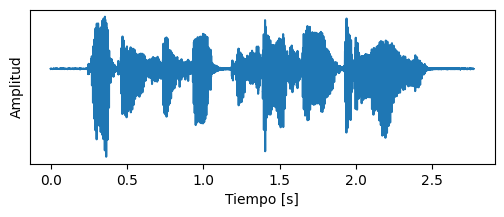
\includegraphics[width=0.75\textwidth]{figures/2.1.waveform.png}
    \caption{Representación de un discurso en el dominio temporal}
    \label{fig:2.1. waveform}
\end{figure}

Por otro lado, la representación en el dominio frecuencial permite visualizar y analizar como se distribuye la energía en el espectro de frecuencias. 

\begin{figure}[h]
    \centering
    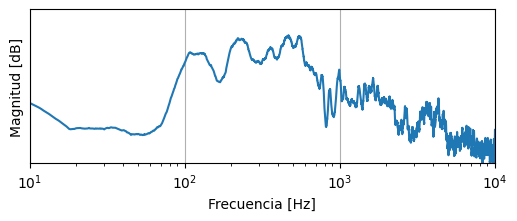
\includegraphics[width=0.75\textwidth]{figures/2.1.spectrum.png}
    \caption{Representación de un discurso en el dominio frecuencial}
    \label{fig:2.1. spectrum}
\end{figure}

Al utilizar la representación temporal del audio, si bien se pueden observar fenómenos energéticos y localizar los mismos en el tiempo, no se puede discernir con solo visualizar la forma de onda si dos señales tienen la misma información o no. Asimismo, al analizar únicamente la representación frecuencial, se pierde la información temporal, la cual es crucial para comprender la dinámica y evolución de la señal a lo largo del tiempo. Para aprovechar la información proporcionada por ambas representaciones, se utilizan las representaciones del tipo tiempo-frecuencia, las cuales permiten analizar cómo evolucionan y cambian los eventos sonoros tanto temporal como frecuencialmente. La representación mas conocida de este tipo es el espectograma, el cual se obtiene a partir de la transformada de Fourier de tiempo corto (STFT, por sus siglas en inglés Short-Time Fourer Transform).


\subsubsection{Transformada de Fourier de tiempo corto (STFT)}
La transformada de Fourier de tiempo corto (STFT) es utilizada para determinar el comportamiento frecuencial y temporal de una señal (\cite{sejdic2009}). En la práctica, el procedimiento para calcular la STFT consiste en tomar pequeños segmentos de la señal a analizar y calcular la transformada de Fourier discreta (DFT, por sus siglas en ingles Discrete Fourier Transform) para cada segmento. Luego, los resultados de la DFT aplicada a cada segmento se agrupan en una matriz compleja, donde las filas representan los bines de frecuencia, y las columnas los segmentos temporales en los que se calculó la DFT. Dado que la transformada de Fourier discreta aplicada a una señal da como resultado una señal compleja, la matriz de la STFT será, a su vez, una matriz compleja. El procedimiento de cálculo tiene algunos detalles y parámetros importantes que modifican el resultado de la transformada, los cuales son:


\begin{itemize}
    \item \textbf{Tamaño de segmento ($M$)}: Todos los segmentos tienen la misma cantidad de muestras, y en base a este parámetro surge una importante relación de compromiso. A medida que se incrementa la cantidad de muestras por segmento, se obtiene una mayor resolución en frecuencia, pero menor resolución temporal, y en contrapartida, al reducir la cantidad de muestras por segmento, se obtiene una mayor resolución temporal a costa de una menor resolución en frecuencia. Generalmente se utilizan valores que sean potencia de 2 (256, 512, 1028) para agilizar el cálculo de la FFT.
    \item \textbf{Tipo de ventana ($w[n]$)}: El procesamiento de los segmentos se suele realizar con un ventaneo previo para evitar los artefactos producidos en los bordes de cada bloque por la discontinuidad de fase. Generalmente se suele utilizar la ventana de Hann.
    \item \textbf{Tamaño de salto ($h$)}: Los segmentos suelen tener un cierto porcentaje de solapamiento en pos de no perder información en sus bordes por culpa del ventaneo. En la práctica, el solapamiento se suele cuantificar con el tamaño de salto entre segmentos (en ingles se conoce como \textit{hop size}). Generalmente se utilizan segmentos con un 50\% de solapamiento, es decir, un tamaño de salto que es la mitad del tamaño de bloque.
\end{itemize}

En la figura \eqref{fig:2.1.stft} se puede ver como interactúan los parámetros mencionados en el procedimiento de cálculo.

\begin{figure}[h]
    \centering
    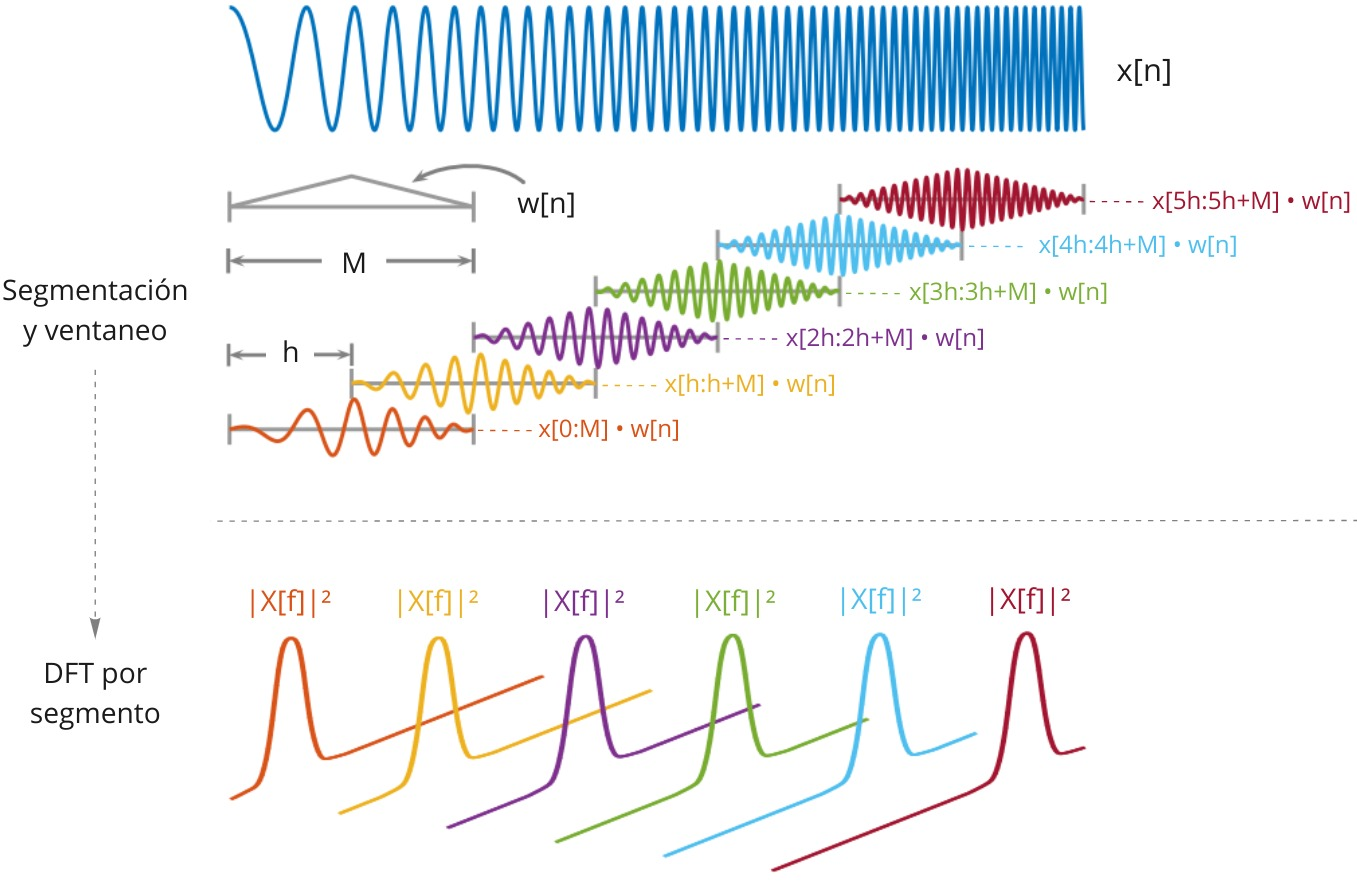
\includegraphics[width=0.95\textwidth]{figures/2.1.stft.jpg}
    \caption{Procedimiento de cálculo de la STFT}
    \label{fig:2.1.stft}
\end{figure}


Matemáticamente, la STFT para una señal discreta $x[n]$ de $M$ muestras se calcula según la ecuación \eqref{eq: stft}:

\vspace{-10mm}

\begin{equation}
    STFT\{x[n]\} = X[k, seg] = \sum \limits_{seg=0}^{N_{seg}} \underbrace{\sum \limits_{k=0}^{M-1} w[n] ~ x[seg\cdot h:seg\cdot h + M] ~ e^{-j2\pi k n / M}}_{\textit{DFT por segmento}}
    \label{eq: stft}
\end{equation}

Por último para obtener el espectrograma de una señal, se debe elevar al cuadrado la magnitud de la STFT ($|X[k, seg]|^2$). Este tipo de representación es de gran utilidad para localizar eventos sonoros tanto temporal como frecuencialmente, pero la mayor información de la voz humana queda concentrada en un rango pequeño del eje frecuencial como se puede ver en la figura \eqref{fig:2.1.spectogram}.

\begin{figure}[h]
    \centering
    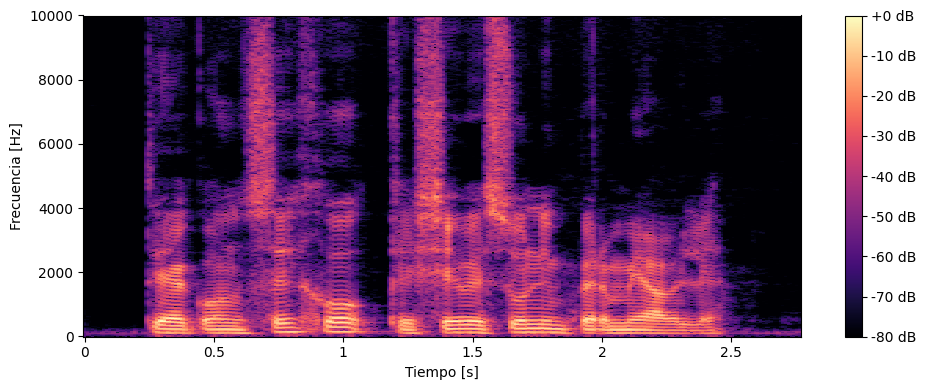
\includegraphics[width=0.85\textwidth]{figures/2.1.spectogram.png}
    \caption{Espectograma del discurso presentado en las figuras \eqref{fig:2.1. waveform} y \eqref{fig:2.1. spectrum}} 
    \label{fig:2.1.spectogram}
\end{figure}

\subsubsection{Espectograma de Mel}

El espectrograma de Mel, similar al espectrograma convencional, es una representación de la energía de una señal de audio en relación con el tiempo y la frecuencia. Sin embargo, se distingue por el mapeo de frecuencias según la escala de Mel, una escala perceptual que refleja cómo los seres humanos perciben las variaciones de tono entre diferentes sonidos. El mapeo para convertir  las frecuencias de la escala convencional $f$ en las frecuencias de la escala Mel $m$ se describe en la ecuación \eqref{eq:2.1.mel_scale}.

\begin{equation}
    m = 2595\log_{10} \Big ( 1 + \frac{f}{700} \Big )
    \label{eq:2.1.mel_scale}
\end{equation}

En la figura \eqref{fig:2.1.mel-spectogram} se puede visualizar el espectograma de Mel aplicado a una señal de habla. En comparativa con el espectograma convencional de la figura \eqref{fig:2.1.spectogram}, se puede notar que se resalta mas el contenido armónico del habla. Este tipo de representación es mas adecuada para  analizar habla ya que se puede observar con mas detalle el rango frecuencial en donde se ubica la voz humana.


\begin{figure}[h]
    \centering
    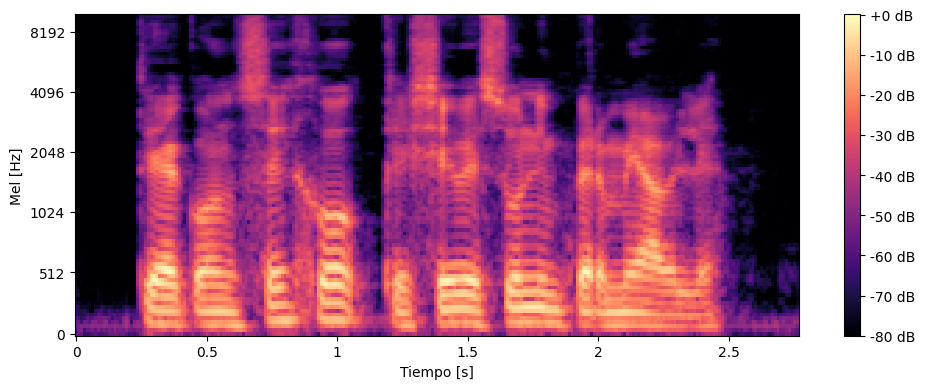
\includegraphics[width=0.85\textwidth]{figures/2.1.mel-spectogram.png}
    \caption{Espectograma de Mel del discurso presentado en las figuras \eqref{fig:2.1. waveform} y \eqref{fig:2.1. spectrum}} 
    \label{fig:2.1.mel-spectogram}
\end{figure}

\subsection{Algoritmos de aprendizaje profundo y redes neuronales artificiales}
Dentro de los algoritmos de aprendizaje profundo, una red neuronal artificial es un modelo matemático inspirado en la estructura y funcionamiento de las neuronas biológicas (\cite{hardesty2017}). En la actualidad, su aplicación se extiende por diversas ramas de la ciencia, y su adopción para la resolución de problemas ha experimentado un crecimiento exponencial en tiempos recientes.

\subsubsection{Neurona artificial}
Una red neuronal artificial se compone de nodos llamados neuronas artificiales, las cuales están interconectadas entre si emulando el proceso de sinapsis (\cite{basheer2000}). En la figura \eqref{fig:2.2.neuron} se puede ver un esquema de los elementos que componen a cada neurona dentro de una red. Cada neurona recibe una determinada señal, la cual procesa y envía a la neurona siguiente. La señal que recibe es una \textbf{serie de números reales} $x_n$, y la salida de cada neurona se calcula mediante una función no lineal aplicada a la suma ponderada de sus entradas, llamada \textbf{función de activación}. La fuerza de la señal en cada conexión es determinada por un \textbf{peso}, que se ajusta durante el proceso de aprendizaje. A su vez, se introduce un término de \textbf{bias} a la suma ponderada, el cual también se actualiza en el proceso de entrenamiento.

\begin{figure}[h]
    \centering
    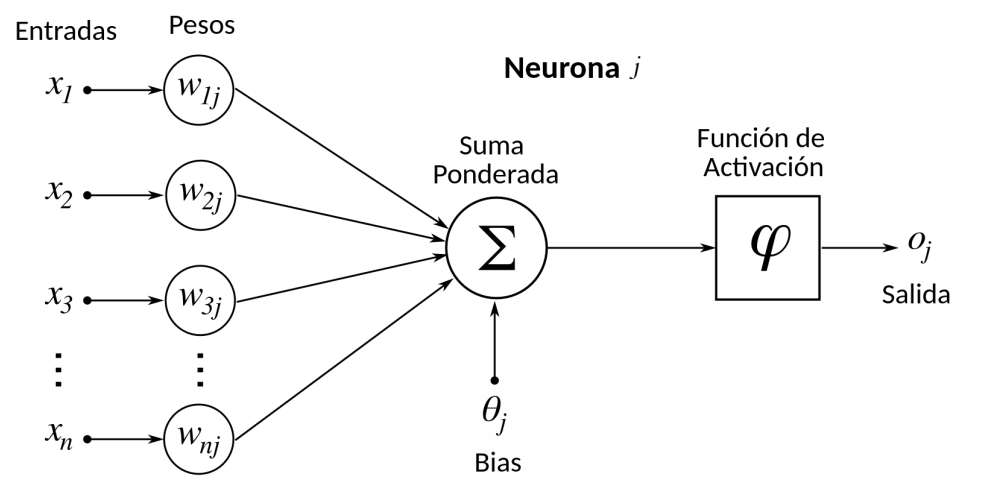
\includegraphics[width=0.85\textwidth]{figures/2.2.neuron.png}
    \caption{Esquema de una neurona artificial} 
    \label{fig:2.2.neuron}
\end{figure}

Este proceso se puede describir matemáticamente con la ecuación \eqref{eq: neuron}.

\begin{equation}
    o_j = \varphi \Big ( \sum \limits_{i=1}^{n}x_i w_{ji} + \theta_j \Big )
    \label{eq: neuron}
\end{equation}

\subsubsection{Redes neuronales artificiales}
Por lo general, las neuronas artificiales se agrupan en \textbf{capas}. Las señales se propagan desde la primera capa (la capa de entrada) hasta la última capa (la capa de salida), pasando por múltiples capas intermedias (capas ocultas). Una red se suele llamar \textbf{red neuronal profunda} si tiene al menos 2 capas ocultas. Esto se debe a que contienen múltiples capas de procesamiento no lineal que aprenden diferentes niveles de representación formando una jerarquía de características, desde un nivel de abstracción más bajo a uno más alto (\cite{chollet2021}). A la hora de construir y diseñar una red neuronal es necesario definir una serie de parámetros que caracterizan como se propaga la señal desde la entrada hasta la salida, como por ejemplo la cantidad de capas, cantidad de neuronas por capa, las funciones de activación, entre otros. Estos parámetros son conocidos como \textbf{hiperparámetros}, ya que se definen a la hora de construir la red pero no se modifican en el proceso de entrenamiento. En la figura \eqref{fig:2.2.net} se puede ver el esquema de una red neuronal profunda básica, la cual está compuesta por 4 capas, una de entrada con 3 neuronas, dos capas ocultas con 5 y 4 neuronas respectivamente, y una de salida con 2 neuronas. Este tipo de red es conocida como perceptron multicapa (\cite{hornik1991}), y a cada nodo se lo denomina perceptron. 


\begin{figure}[h]
    \centering
    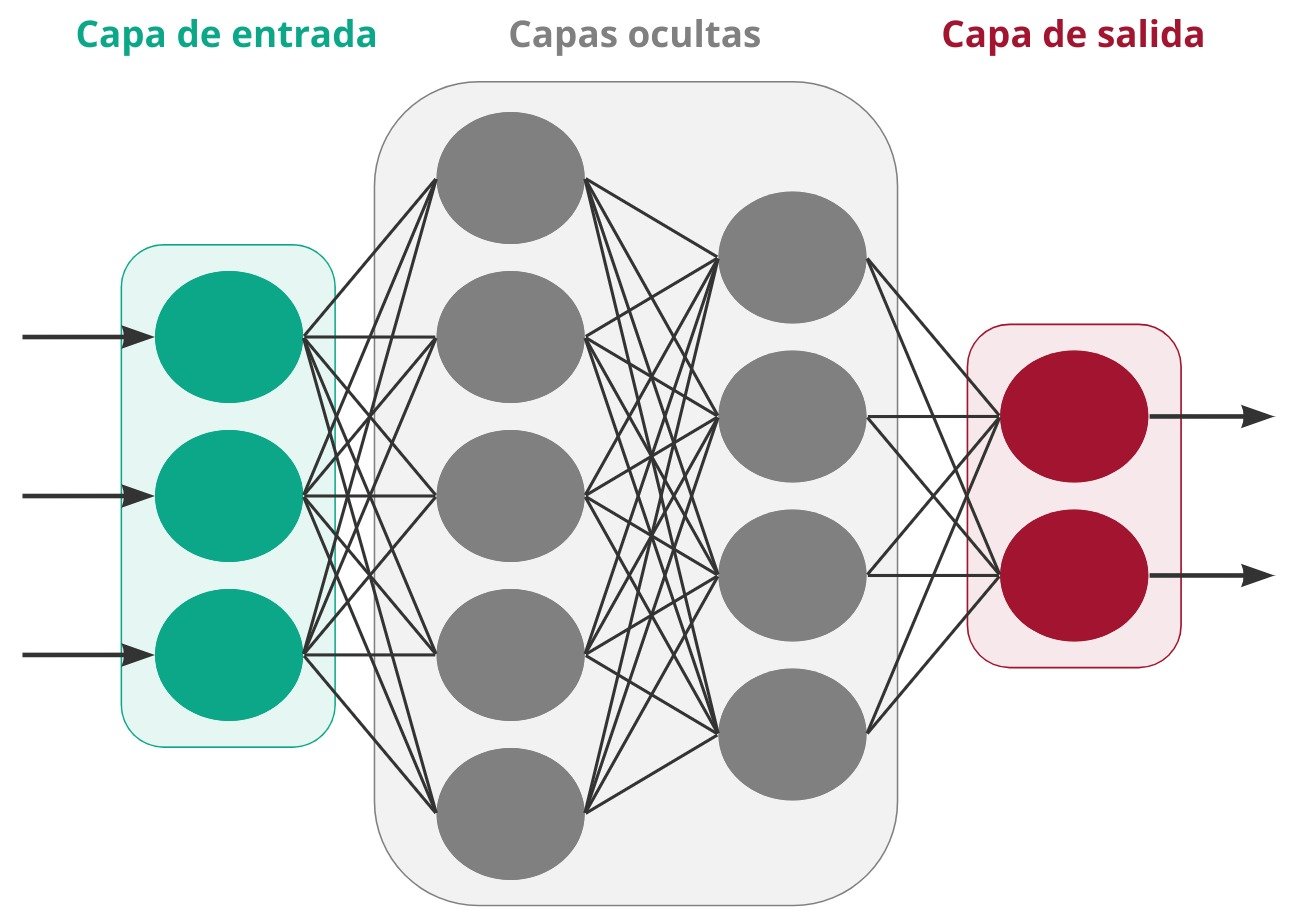
\includegraphics[width=0.7\textwidth]{figures/2.2.net.png}
    \caption{Ejemplo de una red neuronal profunda} 
    \label{fig:2.2.net}
\end{figure}

\subsubsection{Entrenamiento y optimización de modelos}

Los modelos basados en redes neuronales artificiales se dice que ''aprenden'' de los datos producto de un entrenamiento. Este entrenamiento no es mas que un proceso de optimización en el cual se busca que las predicciones del modelo sean lo mas parecidas y cercanas a los valores esperados. Existen diversas formas en las que un modelo puede aprender, siendo la más común denominada aprendizaje supervisado. En este enfoque, los datos de entrenamiento consisten en ejemplos etiquetados que indican cómo debería comportarse el modelo. Esto significa que se le proporciona al modelo tanto los datos de entrada $x$ como las respuestas deseadas $y$ correspondientes. El objetivo es que el modelo aprenda a mapear las entradas a las salidas correctas. En el contexto del entrenamiento de una red neuronal, se define al aprendizaje como la búsqueda de una determinada configuración de los parámetros entrenables $W$ de la red que produzcan que la entrada $x$ genere la salida $y$. En general, al inicio del entrenamiento las entradas van a generar salidas $\hat{y}$ aleatorias que difieren del valor objetivo $y$. Por lo tanto, es necesario tener una medida de esta diferencia. De eso se encarga la función de costo $\mathcal{L}$ (también denominada función de pérdida).

{\large \textbf{Función de costo $\mathcal{L}$}}


La función de costo recibe las salidas de la red $\hat{y}$ y las salidas esperadas $y$, y luego calcula una medida de error a partir de una función matemática. Una de las funciones de costo más conocidas y utilizadas es el error cuadrático medio (MSE, por sus siglas en inglés, Mean Squared Error), que se caracteriza mediante la ecuación \eqref{eq:mse}.

\begin{equation}
    \mathcal{L}(y,\hat{y}) = \frac{1}{N}\sum \limits_{i=1}^{N} (y - \hat{y})^2
    \label{eq:mse}
\end{equation}

La selección de esta función se basa en la característica que se desea analizar y comparar entre las predicciones y los valores esperados. Por lo tanto, para cada estimación de la red, la función de costo otorga un puntaje que explica cuan lejos está el valor estimado del valor objetivo. 

{\large \textbf{Optimización y propagación del error}}

El paso siguiente en el proceso de entrenamiento es utilizar la salida de la función de costo como una señal de realimentación para poder ajustar los parámetros entrenables $W$ de la red neuronal de manera tal de minimizar la función de costo. Esta tarea es realizada por la función de optimización. La misma aplica el algoritmo de propagación del error hacia atrás para computar el gradiente de la función de costo respecto a los parámetros entrenables $W$ de la red. Desde una perspectiva matemática, el gradiente se define como un vector que apunta hacia el punto de máximo crecimiento de una función, mientras que su sentido contrario indica el punto de mínimo crecimiento. Por lo tanto, para minimizar la función de pérdida, es necesario ajustar los parámetros en la dirección opuesta al vector gradiente. A su vez, la fuerza con la que se modifican los parámetros en la dirección opuesta del gradiente se llama tasa de aprendizaje $\eta$. Una vez calculado el gradiente y definida la tasa de aprendizaje $\eta$, se puede determinar cómo modificar los parámetros entrenables $W$ con el fin de reducir el error de salida. Esta operación se puede ver expresada en la ecuación \eqref{eq:learning_rate}.

\begin{equation}
    W := W - \eta \cdot \frac{\partial ~\mathcal{L}}{\partial W}
    \label{eq:learning_rate}
\end{equation}

{\large \textbf{Procesamiento del conjunto de datos}}

En la etapa de entrenamiento, el modelo procesa el conjunto de datos por lotes, es decir, en cada iteración de entrenamiento se toma una muestra sin reposición de un determinado tamaño, se procesa, se calcula la pérdida con la función de costo y
ajusta los parámetros de cada capa. Cuando la red procesó todos los lotes que componen el conjunto de datos de entrenamiento se dice que transcurrió una época. Por ende, tanto el tamaño de los lotes como la cantidad de épocas son hiperparámetros que se definen antes de ejecutar el entrenamiento.

A su vez, el conjunto de datos se divide en tres subconjuntos distintos: conjunto de entrenamiento, conjunto de validación y conjunto de prueba. 

\begin{itemize}
    \item \textbf{Conjunto de entrenamiento:} Este conjunto se utiliza para entrenar el modelo. Es importante que el conjunto de entrenamiento sea lo suficientemente grande y representativo de los datos del mundo real para que el modelo pueda aprender patrones generalizables.
    \item \textbf{Conjunto de validación:} Después de cada iteración de entrenamiento, se utiliza el conjunto de validación para evaluar el rendimiento del modelo.
    \item \textbf{Conjunto de prueba:} Una vez que se ha finalizado el entrenamiento y la validación del modelo, se utiliza el conjunto de prueba para evaluar su rendimiento final de manera objetiva. Este conjunto es completamente independiente del conjunto de entrenamiento y de validación, y no se utiliza en ninguna etapa del proceso de entrenamiento. El conjunto de prueba proporciona una evaluación imparcial del rendimiento del modelo en datos que no ha visto durante el entrenamiento ni la validación. Ayuda a estimar cómo se comportará el modelo en el mundo real.
\end{itemize}

La división de los datos en estos tres conjuntos es fundamental para desarrollar modelos de aprendizaje profundo confiables y generalizables. Ayuda a detectar problemas como sobreajuste (cuando el modelo se ajusta demasiado a los datos de entrenamiento y no generaliza bien) y permite ajustar los hiperparámetros de manera adecuada para obtener un modelo óptimo.

{\large \textbf{Ajuste fino de modelos pre-entrenados}}

En el aprendizaje profundo, el ajuste fino es un enfoque de transferencia de conocimiento en el cual los parámetros de un modelo pre-entrenado son entrenados con nuevos datos (\cite{quinn2020}). El ajuste fino puede realizarse en toda la red neuronal o solo en un subconjunto de sus capas, en cuyo caso las capas que no se están ajustando finamente quedan ''congeladas'' (no se actualizan durante el paso de propagación del error).

\subsection{Breve historia de la síntesis de voz}
Los primeros sistemas de texto a voz, también conocidos como sistemas TTS (por sus siglas en inglés Text-To-Speech), se basaron en métodos computacionales como la síntesis articulatoria, la síntesis de formantes y la síntesis concatenativa. La síntesis articulatoria produce el habla mediante la simulación del comportamiento de los articuladores humanos, como los labios, la lengua, la glotis y el movimiento del tracto vocal, pero tiene una gran limitación, que es muy difícil modelar estos comportamientos de los articuladores en la práctica (\cite{coker1976}). La síntesis de formantes es un tipo de síntesis sustractiva que utiliza picos de frecuencia fija, llamados formantes, para crear el timbre de una voz o instrumento. Este tipo de síntesis es capaz de reproducir discursos inteligibles con poco costo computacional, pero en muchos casos el habla sintética suena menos natural y tiene artefactos artificiales (\cite{seeviour1976}). La síntesis concatenativa se basa en la concatenación de fragmentos de habla que están almacenados en una base de datos. Al igual que la síntesis de formantes, es capaz de reproducir discursos con buena inteligibilidad y con un timbre muy cercano al del sujeto original. Sin embargo, se requiere una enorme base de datos de grabaciones para cubrir todas las posibles combinaciones de unidades de habla. Otra desventaja es que la voz generada es menos natural y emocional, ya que la concatenación puede resultar en una menor suavidad en el énfasis, la emoción y la prosodia (\cite{olive1977}). Posteriormente, con la combinación del aprendizaje automático y la estadística, se propuso la síntesis del habla paramétrica estadística (SPSS, por sus siglas en inglés, Statistical Parametric Speech Synthesis), que predice parámetros y características del discurso como el espectro, la frecuencia fundamental y la duración para utilizarlos en la síntesis (\cite{zen2009}). 
La idea básica es que en lugar de generar directamente la forma de onda a través de la concatenación, primero se generan los parámetros acústicos que son necesarios para producir habla y luego sintetizar el discurso a partir de los parámetros generados. Este tipo de síntesis ofrece ventajas sobre los sistemas anteriores, como una mayor naturalidad en el audio, flexibilidad para modificar parámetros y menor costo de datos al requerir menos grabaciones que la síntesis concatenativa. Sin embargo, también presenta desventajas, como una menor inteligibilidad en el habla generada debido a artefactos como zumbidos o ruidos, y una voz generada que sigue siendo percibida como robótica y fácilmente distinguible del habla humana.


\subsection{Sistemas de texto a voz (TTS) basados en redes neuronales}

A partir del 2010, la síntesis del habla basada en redes neuronales ha ido ganando gradualmente predominancia y ha logrado una calidad de voz mucho mejor. Inicialmente, su adopción comenzó remplazando el módulo de modelado acústico en los sistemas de síntesis paramétrica del habla (SPSS). Sin embargo, en 2016, se presentó WaveNet (\cite{oord2016}), un modelo capaz de generar la forma de onda del discurso a partir de las características lingüísticas del texto, combinando el funcionamiento del modelado acústico y el vocoder en un solo módulo de procesamiento. Este trabajo puede ser considerado como el primer sistema TTS completamente basado en redes neuronales, y la base para muchos trabajos del estado del arte. Por lo general, los sistemas TTS se componen de tres módulos fundamentales, los cuales se muestran en la figura \eqref{fig:2.3.tts-base} y se detallan a continuación.

\begin{figure}[h]
    \centering
    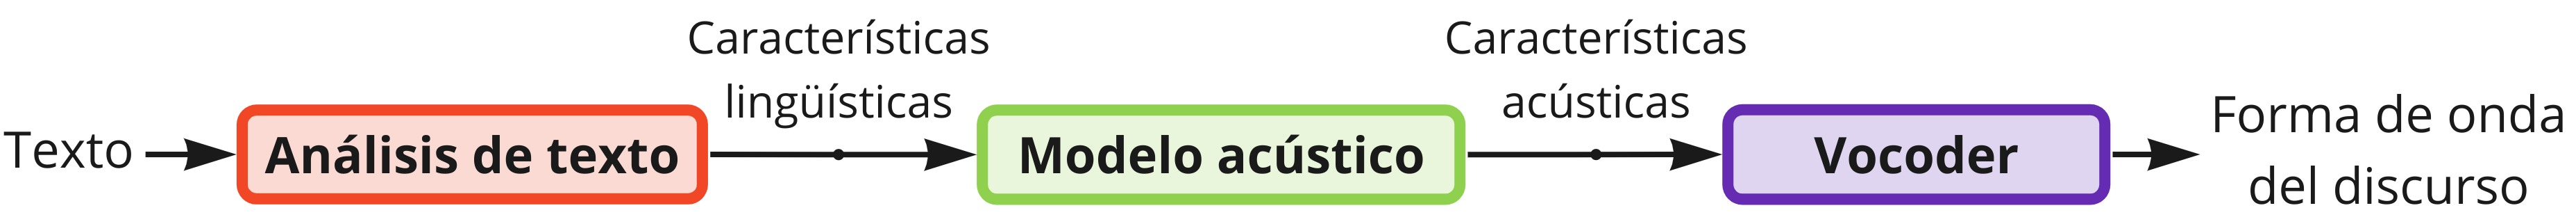
\includegraphics[width=0.95\textwidth]{figures/2.3.tts-base.png}
    \caption{Componentes principales de un sistema de texto a voz (TTS)}
    \label{fig:2.3.tts-base}
\end{figure}

\subsubsection{Análisis de texto}

El módulo de análisis de texto transforma el texto de entrada en características lingüísticas que contienen información detallada sobre la pronunciación y la prosodia. En general, este modulo contiene varias funcionalidades de preprocesamiento del texto, entre ellas:

\begin{itemize}
    \item \textbf{Normalización de texto}: El texto crudo puede contener palabras en formato no estándar que deben convertirse en un formato hablado a través de la normalización de texto. Por ejemplo, el año ''1998'' se normaliza como ''mil novecientos noventa y ocho'', y frases con símbolos específicos como ''82\%'' se normaliza como ''ochenta y dos porciento''. Lo mismo se aplica a las abreviaturas, donde ''Sr.'' o ''Ing.'' se expande a ''señor'' o ''ingeniero'' respectivamente. La normalización puede estar basada en reglas (\cite{sproat2001}), en modelos neuronales (\cite{sproat2016}) o en una combinación de ambos (\cite{zhang2020}).
    
    \item \textbf{Conversión de grafema a fonema}: La conversión de caracteres (grafemas) en pronunciación (fonemas) puede facilitar enormemente la síntesis del habla. Por ejemplo, la palabra ''llamada'' se convierte en ''{\setmainfont{Doulos SIL} /ʎamˈaða/}''. Por lo general, se utiliza un léxico grafema-fonema recopilado manualmente para la conversión. A su vez, el léxico o diccionario recopilado, varía entre los distintos dialectos de un mismo idioma, como por ejemplo con la palabra ''experto'', la cual su conversión a fonemas para el español nativo de España es ''{\setmainfont{Doulos SIL} /esˈpeɾto/}'' pero en el dialecto Rioplatense del Español su conversión es
    ''{\setmainfont{Doulos SIL} /eksˈpeɾto/}''.
\end{itemize}

\subsubsection{Modelo acústico}

\subsubsection{Vocoder}

En general, los sistemas de texto-a-voz o TTS (por sus siglas en inglés Text-To-Speech) basados en redes neuronales cuentan con dos modelos concatenados, uno llamado sintetizador, y el otro vocoder. El sintetizador es el encargado de procesar el texto de entrada para generar una representación del audio correspondiente al habla. Para poder escuchar dicho discurso se utiliza el vocoder, el cual convierte la representación del habla generada por el sintetizador en formas de onda. En particular, el sintetizador es el que debe procesar las características lingüísticas del idioma (pronunciaciones, prosodia, yeísmos) por lo que es el elemento principal de un sistema de TTS a la hora de ajustarlo para un idioma particular. 



Por otro lado se encuentran los sistemas denominados zero-shot (\cite{nvidia2023}), que tienen la capacidad de crear voces que no se han utilizado en su fase de entrenamiento. En dichos sistemas se incluye típicamente un componente adicional conocido como el codificador de hablante (speaker encoder). Este codificador de hablante desempeña un papel esencial al extraer las características acústicas distintivas de una voz específica. Esto se vuelve fundamental en la etapa de inferencia, ya que condiciona la generación de los espectrogramas. En otras palabras, este proceso permite que el sistema extraiga y reproduzca las características primordiales de un hablante, incluso para hablantes que el sistema no procesó durante su fase de entrenamiento.

\begin{figure}[h]
    \centering
    \includegraphics[width=0.8\textwidth]{figures/2.3.tts-zeroshot.jpg}
    \caption{Diagrama de bloques de un sistema TTS con codificador de hablante.}
    \label{fig:2.3.TTS zeros-hot}
\end{figure}

En este estudio, se realiza una comparación exhaustiva entre dos sistemas que están dentro del estado del arte en sistemas de TTS, cada uno de los cuales se caracteriza por la combinación de componentes algorítmicos específicos. La Tabla I desglosa estos sistemas en términos de sus tres componentes principales: el codificador de hablante, el sintetizador, y el Vocoder.

\subsubsection{Sistema 1: GE2E + Tacotron2 + WaveRNN}

Dentro del primer sistema presentado en este estudio, se destaca la utilización del sintetizador Tacotron 2 (\cite{shen2018}). Este opera bajo un enfoque autorregresivo y desempeña un papel fundamental en la transformación de texto en habla articulada. Para comprender cómo se integra este sintetizador en el sistema, la Fig. 1 proporciona un diagrama de bloque ilustrativo. Aquí se esclarece la interconexión de Tacotron 2 con los otros componentes esenciales: el codificador de hablante (Generalized End-to-End (GE2E) (\cite{wan2018})) y el vocoder (WaveRNN (\cite{kalchbrenner2018})).

\begin{figure}[h]
    \centering
    \includegraphics[width=\textwidth]{figures/2.3.tacotron2.jpg}
    \caption{Diagrama de bloques del sistema 1 (GE2E + Tacotron2 + WaveRNN).}
    \label{fig:2.3.tacotron2}
\end{figure}

Dentro del sintetizador, se distinguen tres bloques de procesamiento, cada uno desempeñando un papel crucial en la generación de voz sintética. Estos bloques son: el codificador de texto (Encoder), el modelo de atención (Attention), y el decodificador encargado de la generación de los espectrogramas de Mel (Decoder). 
Debido a la longitud de los espectrogramas y a la naturaleza autorregresiva, este tipo de sistema tiene una serie de desventajas que perjudican su uso en un sistema integral:

\begin{itemize}
    \item Baja velocidad de inferencia en la generación de los espectrogramas: aunque los TTS basados en redes neuronales convolucionales (CNN) pueden acelerar el entrenamiento respecto a los modelos basados en redes neuronales recurrentes (RNN), todos los modelos generan un espectrograma condicionado a los generados previamente (propio de un sistema autorregresivo), por lo que si la secuencia de espectrogramas es larga, el proceso generativo suele ser lento. La condición autoregresiva implica que el sintetizador genera un bloque de espectrograma a la vez, por ende, debe procesar la señal N veces, siendo N el largo del espectrograma (\cite{ren2019}).

    \item El discurso sintetizado no suele ser robusto: Debido a la propagación de errores y a las alineaciones erróneas generadas por el modelo de atención, el espectrograma de Mel generado suele ser deficiente, omitiendo o repitiendo palabras (\cite{wei2018}).

    \item Carencia de control a la hora de generar discursos: Los modelos autorregresivos generan de a bloques de espectrograma uno a uno de forma automática, sin aprovechar las alineaciones entre texto y habla. Como consecuencia, suele ser difícil controlar directamente la velocidad y la prosodia de la voz en la generación autorregresiva. 
    
\end{itemize}

\subsubsection{Sistema 2: FastPitch + HiFiGAN}

Una estrategia que acelera la generación de espectrogramas contempla el uso de sintetizadores que operen en paralelo, tal como lo hace el sintetizador FastPitch (\cite{lancucki2021}). Este sintetizador se basa en la tecnología Transformer y se distingue por su enfoque de generación de espectrogramas que no sigue un proceso autorregresivo. En lugar de ello, FastPitch adopta un enfoque de generación paralela. Una característica destacada es su capacidad para trabajar directamente con los fonemas del texto, lo que implica el uso de un conversor de grafemas a fonemas antes de ingresar el texto al sistema. La arquitectura de FastPitch, representada en la Fig. 2, se compone de dos bloques feed-forward Transformer (FFTr) (\cite{ren2019}) y módulos que predicen tanto el pitch como la duración para cada fonema del texto. Este enfoque de paralelismo y la integración de predictores de pitch y duración contribuyen a la velocidad y precisión del proceso de síntesis de voz.

\begin{figure}[h]
    \centering
    \includegraphics[width=\textwidth]{figures/2.3.fastpitch.jpg}
    \caption{Diagrama de bloques del sistema 2 (FastPitch + HiFiGAN).}
    \label{fig:2.3.fastpitch}
\end{figure}

Gracias al módulo de predicción de duración de fonemas, se garantiza que la alineación entre un fonema y su espectrograma asociado sea robusta. De esta forma se evita la propagación de errores y alineaciones erróneas, reduciendo en consecuencia la proporción de palabras omitidas y/o repetidas. A diferencia del Sistema 1, el Sistema 2 no opera en modo zero-shot, sino que es un sistema de síntesis de voz personalizado. En otras palabras, esto significa que, si se desea crear una copia de una voz específica, se necesita volver a entrenar el sintetizador utilizando los datos de la persona cuya voz se quiere replicar. El Sistema 2 no tiene la capacidad de adaptarse automáticamente a las características vocales de un nuevo hablante durante el proceso de inferencia. Por último, en este sistema se utiliza el vocoder HiFiGAN (\cite{kong2020}), el cual genera audio de alta calidad a gran velocidad a partir de espectrogramas de mel con redes generativas adversariales.
En los sistemas tratados anteriormente, fueron detalladas las arquitecturas de los sintetizadores ya que son responsables de adoptar las características lingüísticas del idioma. Para el caso de los Vocoders, el idioma de los datos utilizados en el entrenamiento tiene un efecto mínimo. Cómo el principal objetivo del Vocoder es lograr un audio de calidad a partir de un cierto espectrograma, resulta conveniente valerse de un modelo entrenado con una extensa cantidad de datos, aunque se haya implementado en un idioma distinto al que se va a utilizar.
Actualmente no hay desarrollos de estas tecnologías especializadas en el dialecto rioplatense del español. La gran mayoría de modelos de generación de habla son diseñados principalmente para el idioma inglés, y luego se adapta a español nativo. Si bien los modelos en español son ampliamente utilizados, no son capaces de representar los modismos, yeísmos y contenidos prosódicos del dialecto mencionado.


\subsection{Parámetros objetivos de calidad, similitud e inteligibilidad}

Para realizar un estudio enfocado en los discursos sintetizados, se busca evaluar el sistema con diversos parámetros que determinen la calidad, la similitud con la voz objetivo y la naturalidad de la narración generada. A continuación, se detallan los parámetros que se tomarán en cuenta para el análisis, acompañados de una breve descripción de su significado y la cualidad del discurso que buscan caracterizar:

\subsubsection{Evaluación perceptiva de la calidad del habla (PESQ)}

La evaluación perceptiva de la calidad del habla, conocida como PESQ (\cite{rix2001}) (por sus siglas en inglés Perceptual Evaluation of Speech Quality), conforme a la normativa ITU-T P.862 (\cite{itu-p862}), es un estándar internacional empleado para evaluar la calidad de la voz en el ámbito de las telecomunicaciones, el cual proporciona una puntuación que varía de -0.5 a 4.5, donde valores más altos indican mejor calidad. Esta medida realiza su evaluación comparando la señal de habla original con la señal que ha sido transmitida o procesada, característica que lo define como un método intrusivo. La ITU, debido a la complejidad del procedimiento y al hecho de que PESQ es un estándar patentado, no divulga una fórmula explícita para su cálculo. No obstante, se sugiere la implementación de un enfoque no intrusivo para su cálculo, es decir, uno que no requiera acceso al discurso original, sino que permita realizar el cálculo directamente sobre el discurso sintético. Para este fin, se considera el uso de la librería de Python TorchAudio-Squim (\cite{kumar2023}), la cual mediante un modelo de aprendizaje profundo, ofrece una estimación precisa de la métrica en cuestión. 

\subsubsection{Ingeligibilidad objetiva de tiempo corto (STOI)}

La inteligibilidad objetiva de tiempo corto, también conocida como STOI (\cite{taal2010}) (por sus siglas en inglés Short-Time Objective Intelligibility) mide la inteligibilidad del habla, es decir, qué tan bien se pueden comprender las palabras en condiciones de ruido o procesamiento de señal. La puntuación varía de 0 a 1, donde 1 indica perfecta inteligibilidad. Matemáticamente, STOI compara la correlación entre las envolventes temporales de la señal original y la señal procesada en bandas de frecuencia críticas. En este caso, y al igual que en el caso del PESQ, se propone utilizar TorchAudio-Squim para realizar el cálculo de forma no intrusiva.

\subsubsection{Relación señal a distorsión invariante a la escala (SI-SDR)}

La relación de señal a distorsión invariante a la escala (\cite{leroux2019}) (SI-SDR, por sus siglas en inglés) es una métrica empleada para evaluar el rendimiento de algoritmos de separación de fuentes de habla y audio. Esta mide la mejora en la calidad de la señal separada respecto a la mezcla original, considerando la invarianza de escala de las señales de audio. El SI-SDR es una métrica más robusta y significativa que el SDR tradicional, especialmente para escenarios donde el escalado temporal es desconocido. Su unidad de medida es el dB, donde un valor más alto de SI-SDR señala una menor presencia de distorsión en el contenido del audio, y valores cercanos a 0 dB denotan una alta presencia de distorsión y ruido. Al igual que en el caso del PESQ y del STOI, se sugiere realizar el cálculo de forma no intrusiva, ya que en este caso de aplicación no hay un par de audios a comparar, si no que simplemente se busca evaluar la calidad del audio generado.

\subsubsection{Evaluación no intrusiva de la calidad del habla (NISQA)}

La evaluación no intrusiva de la calidad del habla, también conocida como NISQA (\cite{mittag2021}) (por sus siglas en inglés, Non-Intrusive Speech Quality Assessment), se basa en un modelo de aprendizaje profundo diseñado para predecir la calidad del habla. Se emplea para evaluar y calificar sistemas de mejora del habla, canales de transmisión de audio y sistemas de habla sintética. El valor que reporta es una predicción del MOS (por sus siglas en ingles Mean Opinion Score), por lo que oscila entre 1 y 5. Su aplicación como método de evaluación es ampliamente utilizada (\cite{hasanabadi2023mfccgan}) en el estado del arte de los sistemas de habla sintética, haciéndolo esencial para comparaciones con implementaciones de vanguardia.

\subsubsection{Similitud coseno entre vectores de características}

Para medir la similitud entre la voz generada y la voz objetivo, se sugiere analizar la similitud o distancia entre vectores que representen las características acústicas de ambas voces. Esto implica procesar tanto los discursos sintéticos como los originales con un extractor de características de hablante. Este tipo de modelo es comúnmente utilizado para comprobar si dos discursos son de la misma persona o no (conocidos como sistemas de verificación de hablante), por lo que el vector de características que extrae es sumamente informativo sobre las características tonales y prosódicas de los hablantes. Con los vectores extraídos, es posible comparar objetivamente la similitud entre dos voces calculando la distancia coseno que hay entre ambos vectores. Esta métrica reporta valores entre 0 y 1, donde 1 indica que ambos vectores tienen la misma dirección y sentido, lo cual sugiere una gran similitud entre las voces. En este caso, se propone utilizar el modelo de extracción de características de hablante TitaNet (\cite{koluguri2022}), el cual fue entrenado para identificar si dos discursos son de la misma persona o no.

\subsubsection{Distancia de Frechet entre representaciones de audio (FAD)}
TODO

\subsubsection{Precisión de palabra (WAcc)}
TODO

Estas tres áreas de análisis (calidad, similitud y naturalidad) se buscan validar mediante una evaluación subjetiva. Con ambas evaluaciones se propone realizar un análisis estadístico con el fin de caracterizar la percepción subjetiva basada en los parámetros descritos.

\subsection{Audiolibros}
Un audiolibro es básicamente la grabación de la narración de un libro.
Gracias al avance de las nuevas tecnologías en el ámbito de la información y la distribución de contenidos, su popularidad ha crecido notablemente, consolidándose como el ''cuarto formato'' del libro digital (\cite{bencomo2022}). El audiolibro emerge como un medio de comunicación esencial en situaciones donde la lectura directa no es posible de efectuar. Ofrece una vía para preservar materiales que de otro modo podrían deteriorarse o extraviarse. Su formato posibilita la realización de diversas actividades simultáneas, como conducir, caminar, tomar sol o cocinar. Su accesibilidad, tanto en términos de descarga como de ejecución, y su relativa economía lo convierten en una alternativa atractiva. La narración puede ser generada de forma artificial o realizada por lectores humanos, frecuentemente actores capacitados para ello. En el ámbito comercial, los audiolibros suelen contar con narradores profesionales que ofrecen una interpretación y dramatización de los textos. Algunas editoriales ofrecen opciones de personalización, como la elección entre voces femeninas o masculinas, distintas variedades de español o inglés, así como la posibilidad de seleccionar el tono, timbre y cadencia de los locutores. En la actualidad existen diversas plafatormas en línea como Audible (\cite{audible}) o Libro.fm (\cite{librofm}), sin embargo, ambas requieren suscripción y no ofrecen la capacidad de producir contenido personalizado de manera directa. Por otro lado, existen alternativas como Eleven Labs (\cite{elevenlabs}) la cual posibilita la generación de habla sintética de alta calidad en varios idiomas, con la opción de personalizar los discursos según las necesidades del usuario. Aunque esta plataforma se destaca por su enfoque en la síntesis del habla, también ofrece funcionalidades para la creación sencilla de audiolibros. No obstante, es importante señalar que opera bajo un esquema de suscripción mensual.